% 固定来源第1页中栏Q14：原图标号、三条隐藏棱、AM/CN。
% 平行投影为绘图参数；中点关系由实际投影坐标精确保留。
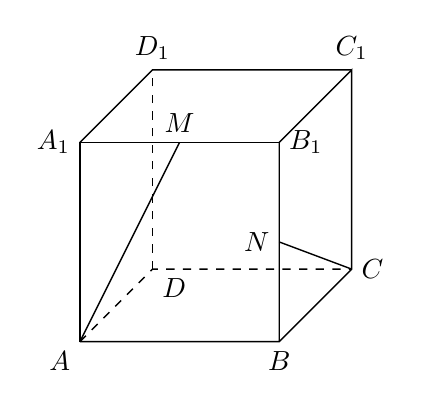
\begin{tikzpicture}[line width=0.5pt,scale=1.15]
  \coordinate (A) at (0,0);
  \coordinate (B) at (2.2,0);
  \coordinate (C) at (3,0.8);
  \coordinate (D) at (0.8,0.8);
  \coordinate (A1) at (0,2.2);
  \coordinate (B1) at (2.2,2.2);
  \coordinate (C1) at (3,3);
  \coordinate (D1) at (0.8,3);
  \coordinate (M) at (1.1,2.2);
  \coordinate (N) at (2.2,1.1);
  \draw (A)--(B)--(C)--(C1)--(B1)--(B);
  \draw (A)--(A1)--(B1);
  \draw (A1)--(D1)--(C1);
  \draw[dashed] (A)--(D)--(C);
  \draw[dashed] (D)--(D1);
  \draw (A)--(M);
  \draw (C)--(N);
  \node[below left] at (A) {$A$};
  \node[below] at (B) {$B$};
  \node[right] at (C) {$C$};
  \node[below right] at (D) {$D$};
  \node[left] at (A1) {$A_1$};
  \node[right] at (B1) {$B_1$};
  \node[above] at (C1) {$C_1$};
  \node[above] at (D1) {$D_1$};
  \node[above] at (M) {$M$};
  \node[left] at (N) {$N$};
\end{tikzpicture}
